%* 
%* ------------------------------------------------------------------
%* CTCPanels.tex - Creating CTC Panels
%* Created by Robert Heller on Thu Apr 19 14:37:54 2007
%* ------------------------------------------------------------------
%* Modification History: $Log$
%* Modification History: Revision 1.2  2007/10/22 17:17:27  heller
%* Modification History: 10222007
%* Modification History:
%* Modification History: Revision 1.1  2007/05/06 12:49:38  heller
%* Modification History: Lock down  for 2.1.8 release candidate 1
%* Modification History:
%* Modification History: Revision 1.1  2002/07/28 14:03:50  heller
%* Modification History: Add it copyright notice headers
%* Modification History:
%* ------------------------------------------------------------------
%* Contents:
%* ------------------------------------------------------------------
%*  
%*     Model RR System, Version 2
%*     Copyright (C) 1994,1995,2002-2005  Robert Heller D/B/A Deepwoods Software
%* 			51 Locke Hill Road
%* 			Wendell, MA 01379-9728
%* 
%*     This program is free software; you can redistribute it and/or modify
%*     it under the terms of the GNU General Public License as published by
%*     the Free Software Foundation; either version 2 of the License, or
%*     (at your option) any later version.
%* 
%*     This program is distributed in the hope that it will be useful,
%*     but WITHOUT ANY WARRANTY; without even the implied warranty of
%*     MERCHANTABILITY or FITNESS FOR A PARTICULAR PURPOSE.  See the
%*     GNU General Public License for more details.
%* 
%*     You should have received a copy of the GNU General Public License
%*     along with this program; if not, write to the Free Software
%*     Foundation, Inc., 675 Mass Ave, Cambridge, MA 02139, USA.
%* 
%*  
%* 

\chapter{Creating CTC Panels}
\label{chapt:CTCPanels}
\typeout{$Id$}

Version 2 of the CTC Panel code is covered in this chapter.  Version 1
is depreciated and is included only for older applications.

\section{Creating a CTCPanel and creating objects to populate it.}
\begin{lstlisting}[caption={CTCPanel::CTCPanel procedure},
		   label={lst:CTC:CTCPanelproc}]
CTCPanel::CTCPanel widgetpath [options...]
\end{lstlisting}
CTCPanels are implemented with a Snit widget type and are created with
the CTCPanel::CTCPanel procedure, as shown in
Listing~\ref{lst:CTC:CTCPanelproc}. This widget takes four options:
\begin{description}\index{CTCPanels!options}
\item[-schematicbackground] The background color of the schematic
display. Defaults to black.
\item[-controlbackground] The background color of the control display.
Defaults to darkgreen.
\item[-width] The total width of the megawidget.
\item[-height] The total height of the megawidget.
\end{description}
\begin{lstlisting}[caption={CTCPanel::CTCPanel creating objects},
		   label={lst:CTC:CTCPanelcreate}]
$CTCPanelObject create type name [options...]
\end{lstlisting}
\begin{table}[hbpt]
\begin{centering}
\begin{tabular}{|l|p{3in}|}
\hline
Method & Description \\
\hline
\hline
getv & Gets the current value of the object.\\
\hline
setv & Set the value of the object.\\
\hline
geti & Gets the value of the specified indicator. \\
\hline
seti & Sets the value of the specified indicator. \\
\hline
itemcget & Gets the value of a specified option of the object.\\
\hline
itemconfigure & Sets the value of a specified option of the object.\\
\hline
exists & Tests to see of the object exists.\\
\hline
delete & Deletes the specified object.\\
\hline
move & Moves the specified object a relative distance.\\
\hline
class & Returns the class (or type) of the object.\\
\hline
invoke & Executes a script bound to an object.\\
\hline
coords & Returns the coordinates of a specified terminal element of the
object. \\
\hline
print & Writes a scriptlet to re-create the object to the specified
output stream.\\
\hline
\end{tabular}
\caption{Object methods}\index{CTCPanels!object methods}
\label{tab:CTC:ObjectMethods}
\end{centering}
\end{table}
The panel includes its own scrollbars, including a shared horizontal
scrollbar. Items displayed on the CTCPanel (either as schematic
trackwork in the schematic display or as control items in the control
display) are created with the create command, as shown in
Listing~\ref{lst:CTC:CTCPanelcreate}.  Each object has a unique name, a
value, zero or more indicators, and zero or more options.  The CTCPanel
widget defines thirteen methods that take an object name, as shown in
Table~\ref{tab:CTC:ObjectMethods}. 

\section{Control Points}

Objects on a CTCPanel are grouped into named Control Points.  A Control
Point defines one (or more) trackwork elements and their corresponding
control panel elements.  In the simplest case a control point might
include a Switch (turnout), a SIGPlate, a SWPlate, and a CodeButton,
with the SWPlate controlling the Switch and the SIGPlate controlling the
signals surrounding the Switch.

\section{Object values and invocation}

Many objects have an associated value.  Generally, these values
represent state information and these values (or states) correspond to
different scripts bound to the object.  For example trackwork switches
(turnouts) define their state as being normal (points aligned for the
main line) or reversed (points aligned for the branch line).

Also many objects have \lstinline=-command= options, which define
scriptlets to invoke under certain conditions.  One (or more) of these
scriptlets are executed (at the global level) when the object is
invoked.  Generally, trackwork objects are invoked to acquire state
information (such as occupancy or point state feedback) from input
ports bits (such as read from a Chubb CMR/I serial bus), and control
objects are invoked to read and effect control panel settings by
setting output port bits for trackwork control and signals.  Generally,
the \lstinline=-command= bound to a code button will in turn invoke all
of the objects associated with the control point the code button
manages.

All trackwork objects have an \lstinline=-occupiedcommand= option,
which is a script to run to fetch the object's occupied state.  The
invoke method always returns the occupied state (always false for
objects that are not trackwork objects).  Trackwork with movable points
should not have their points moved which a train is occupying the
trackwork!  Generally, if any of the trackwork of a control point is
occupied, the control point's code button should not invoke any of the
control elements.

\section{Sample CTCPanel and the code to create it.}

\lstinputlisting[caption={Creating a CTC Panel},
		 label={lst:CTC:CTCPanelCode},
		 firstline=36]{SampleCodeCTCPanel.tcl}
\begin{figure}[hbpt]
\begin{centering}
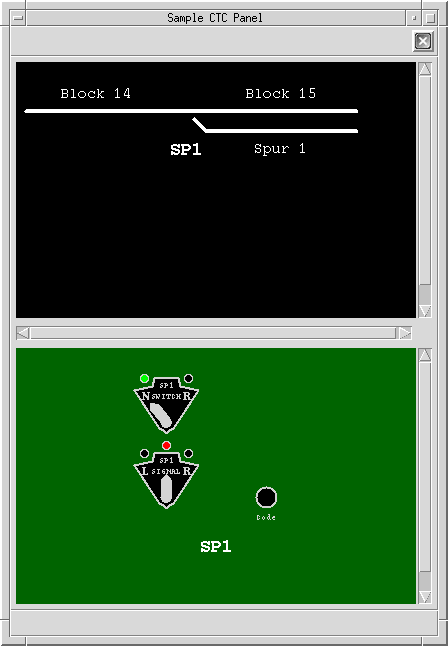
\includegraphics{CTCPanel.png}
\caption{Sample CTC Panel Screen Shot}
\label{fig:CTC:CTCPanelWindow}
\end{centering}
\end{figure}
The Tcl  code in Listing~\ref{lst:CTC:CTCPanelCode} creates a simple
CTC Panel\footnote{See~\cite{internals}, Section 1.4 for a complete
list of available panel elements.}. The CTC Panel itself is created at
line 61 Lines 67--192 populate the panel with both control panel
elements and track schematic elements.  The panel is shown in
Figure~\ref{fig:CTC:CTCPanelWindow}.  

This CTC Panel features a switch (turnout) off the main line to an
industrial spur. There is one actual control point, named SP1, and
three blocks, two for the mainline blocks and one for the industrial
spur.  I have put each block into a separate logical control point as a
organizational  convenience.  The control point SP1 contains one piece
of trackwork, the switch, and four control panel items, a switch plate,
a signal plate, a code button, and a label.  The code does not interact
with an actual layout.  Normally, the \lstinline=-occupiedcommand= 
options of the trackwork elements would define code to read block
occupancy detectors and the \lstinline=-statecommand= of the switch
would define code to read the switch's point position feedback
sensors\footnote{Using the  CMR/I (Bruce Chubb) Interface, as described
in Chapter~\ref{chapt:CMRI:CMRIProgramming}, for example.}. The code
for the switch plate (procedure SetSwitchSP1) would just set the output
bits to activate the switch's switch machine.  The signal plate code
(procedure SetSignalSP1) would also set the output bits to update the
aspects of the signals protecting the switch.

